%!TEX root = ../egpaper_for_review.tex

\tikzstyle{nS}=[circle,minimum size = 0.6cm,inner sep = 0pt,draw, font=\small,align=left]
\tikzstyle{eS}=[thick,minimum size = 0.5cm,inner sep = 0pt,draw, font=\small,align=left]
\tikzstyle{eC}=[very thick,minimum size = 0.5cm,inner sep = 0pt,draw=red, font=\small,align=left]
\tikzstyle{eNC}=[very thick,minimum size = 0.5cm,inner sep = 0pt,draw=green, font=\small,align=left]
\tikzstyle{eNS}=[fill=white,minimum size = 0.5cm,inner sep = 0pt, font=\tiny,align=left]
\tikzstyle{eCC}=[very thick,dotted,minimum size = 0.5cm,inner sep = 0pt,draw=black, font=\small,align=left]

\begin{center}
\begin{figure}[h]
\begin{subfigure}[t]{0.4\linewidth}
    \resizebox{\linewidth}{!}{
        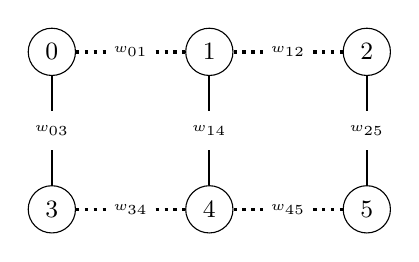
\begin{tikzpicture}[scale=1]%[x=1 cm, y=1 cm]
                \draw (2,2) node[nS] (n0) {$0$}; 
                \draw (4,2) node[nS] (n1) {$1$};
                \draw (6,2) node[nS] (n2) {$2$};
                \draw (2,0) node[nS] (n3) {$3$}; 
                \draw (4,0) node[nS] (n4) {$4$};
                \draw (6,0) node[nS] (n5) {$5$};
                \path
                    (n0) edge[eCC] node[eNS]{$w_{01}$} (n1) 
                    (n1) edge[eCC] node[eNS]{$w_{12}$} (n2) 
                    (n3) edge[eCC] node[eNS]{$w_{34}$} (n4) 
                    (n4) edge[eCC] node[eNS]{$w_{45}$} (n5)
                    (n0) edge[eS] node[eNS]{$w_{03}$} (n3)
                    (n1) edge[eS] node[eNS]{$w_{14}$} (n4)
                    (n2) edge[eS] node[eNS]{$w_{25}$} (n5)
                ;
        \end{tikzpicture}
    }
\caption{ consistent edge labeling $y$ on $G$}
\label{fig:cont_a}
\end{subfigure}
\hfill
\begin{subfigure}[t]{0.4\linewidth}
    \resizebox{\linewidth}{!}{
        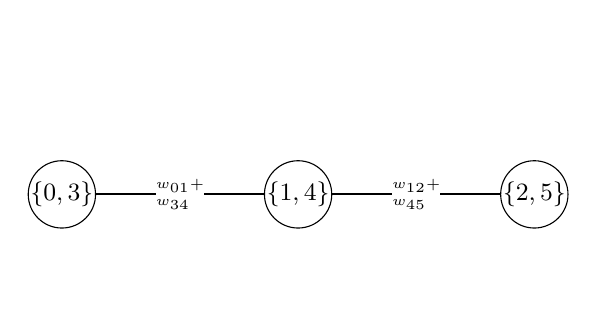
\begin{tikzpicture}[scale=1]%[x=1 cm, y=1 cm]
                \draw (0,1) node[nS] (n0) {$\{0,3\}$}; 
                \draw (3,1) node[nS] (n1) {$\{1,4\}$};
                \draw (6,1) node[nS] (n2) {$\{2,5\}$};
                \draw (0,0) node (d) {}; 
                \draw (0,3) node (d) {}; 
                %\draw (2,0) node[nS] (n3) {$3$}; 
                %\draw (4,0) node[nS] (n4) {$4$};
                %\draw (6,0) node[nS] (n5) {$5$};
                \path
                    (n0) edge[eS] node[eNS]{$w_{01}+$\\$w_{34}$} (n1) 
                    (n1) edge[eS] node[eNS]{$w_{12}+$\\$w_{45}$} (n2) 
                    %(n3) edge[eCC] node[eNS]{$w_{34}$} (n4) 
                    %(n4) edge[eCC] node[eNS]{$w_{45}$} (n5)
                    %(n0) edge[eS] node[eNS]{$w_{03}$} (n3)
                    %(n1) edge[eS] node[eNS]{$w_{14}$} (n4)
                    %(n2) edge[eS] node[eNS]{$w_{25}$} (n5)
                ;
        \end{tikzpicture}
    }
\caption{ {contraction graph $G_y$ given $y$  }}
\label{fig:cont_b}
\end{subfigure}
\\
\begin{subfigure}[t]{0.4\linewidth}
    \resizebox{\linewidth}{!}{
        \begin{tikzpicture}[scale=1]%[x=1 cm, y=1 cm]
                \draw (0,1) node[nS] (n0) {$\{0,3\}$}; 
                \draw (3,1) node[nS] (n1) {$\{1,4\}$};
                \draw (6,1) node[nS] (n2) {$\{2,5\}$};
                \draw (0,0) node (d) {}; 
                \draw (0,3) node (d) {}; 
                %\draw (4,0) node[nS] (n4) {$4$};
                %\draw (6,0) node[nS] (n5) {$5$};
                \path
                    (n0) edge[eS] node[eNS]{$w_{01}+$\\$w_{34}$} (n1) 
                    (n1) edge[eCC] node[eNS]{$w_{12}+$\\$w_{45}$} (n2) 
                    %(n3) edge[eCC] node[eNS]{$w_{34}$} (n4) 
                    %(n4) edge[eCC] node[eNS]{$w_{45}$} (n5)
                    %(n0) edge[eS] node[eNS]{$w_{03}$} (n3)
                    %(n1) edge[eS] node[eNS]{$w_{14}$} (n4)
                    %(n2) edge[eS] node[eNS]{$w_{25}$} (n5)
                ;
        \end{tikzpicture}
    }
\caption{ cut $y^*$ on contraction graph $G_w$ }
\label{fig:cont_c}
\end{subfigure}
\hfill
\begin{subfigure}[t]{0.4\linewidth}
    \resizebox{\linewidth}{!}{
        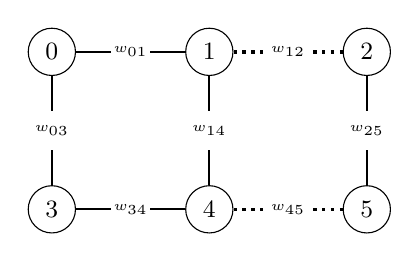
\begin{tikzpicture}[scale=1]%[x=1 cm, y=1 cm]
                \draw (2,2) node[nS] (n0) {$0$}; 
                \draw (4,2) node[nS] (n1) {$1$};
                \draw (6,2) node[nS] (n2) {$2$};
                \draw (2,0) node[nS] (n3) {$3$}; 
                \draw (4,0) node[nS] (n4) {$4$};
                \draw (6,0) node[nS] (n5) {$5$};
                \path
                    (n0) edge[eS] node[eNS]{$w_{01}$} (n1) 
                    (n1) edge[eCC] node[eNS]{$w_{12}$} (n2) 
                    (n3) edge[eS] node[eNS]{$w_{34}$} (n4) 
                    (n4) edge[eCC] node[eNS]{$w_{45}$} (n5)
                    (n0) edge[eS] node[eNS]{$w_{03}$} (n3)
                    (n1) edge[eS] node[eNS]{$w_{14}$} (n4)
                    (n2) edge[eS] node[eNS]{$w_{25}$} (n5)
                ;
        \end{tikzpicture}
    }
\caption{ cut $y^*$ projected on $G$}
\label{fig:cont_d}
\end{subfigure}
\hfill
\caption{
Given a graph $G=(V, E, w)$ and a consistent edge labeling $y$ (fig.~\ref{fig:cont_a}), the contraction 
graph  $G_y=(V_y,E_y, w_y) $ is constructed by contracting each uncut edge in $G$ w.r.t. $y$ (fig.~\ref{fig:cont_b}).
Edge weights in $G_y$ are sum of edges between the connected components (???).
A cut $y^*$ defined on $G_y$  (fig.~\ref{fig:cont_c}) can be projected to $G$ (fig.~\ref{fig:cont_d}).
}\label{fig:contraction}
\end{figure}
\end{center}



